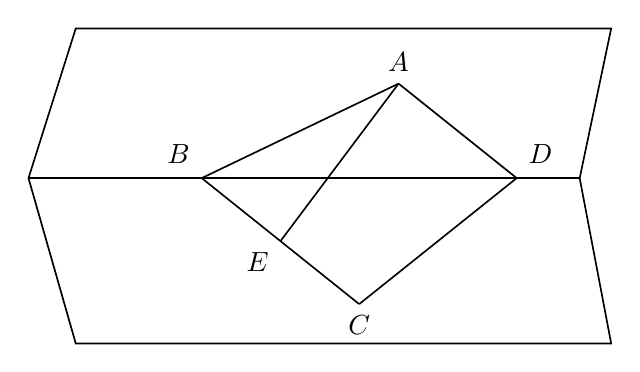
\begin{tikzpicture}[x=1cm,y=1cm,font=\normalsize,line width=.6pt]
\coordinate (B) at (-2,0);
\coordinate (D) at (2,0);
\coordinate (A) at (0.5,1.2);
\coordinate (C) at (0,-1.6);
\coordinate (E) at (-1,-0.8);
\coordinate (TL) at (-3.6,1.9);
\coordinate (TR) at (3.2,1.9);
\coordinate (BL) at (-3.6,-2.1);
\coordinate (BR) at (3.2,-2.1);
\coordinate (L) at (-4.2,0);
\coordinate (R) at (2.8,0);
% upper plane outline
\draw (L) -- (TL) -- (TR) -- (R);
% lower plane outline
\draw (L) -- (BL) -- (BR) -- (R);
% fold / intersection line BD extended
\draw (L) -- (R);
% tetrahedron edges
\draw (A) -- (B);
\draw (A) -- (D);
\draw (B) -- (C);
\draw (C) -- (D);
\draw (A) -- (E);
% labels clear of strokes
\node[inner sep=2pt,anchor=south] at ([yshift=2pt]A) {$A$};
\node[inner sep=2pt,anchor=south east] at ([xshift=-2pt,yshift=3pt]B) {$B$};
\node[inner sep=2pt,anchor=south west] at ([xshift=2pt,yshift=3pt]D) {$D$};
\node[inner sep=2pt,anchor=north] at ([yshift=-2pt]C) {$C$};
\node[inner sep=2pt,anchor=north east] at ([xshift=-2pt,yshift=-2pt]E) {$E$};
\end{tikzpicture}
